%------------------------------------------------------------------------------------
%	CHAPTER 2
%------------------------------------------------------------------------------------
\chapterimage{headConceito.png}
\chapter{Conceitos Introdutórios}

\begin{remark}
A melhor forma de prever o futuro é cria-lo. (Peter Drucker - Escritor e Pai da Administração Moderna) 
\end{remark}

\section{Termos da Estatística}\index{Conceitos Introdutórios}
Devemos sempre possuir um vocabulário comum, e mesmo que não se entenda absolutamente nada de estatística (e tenha um Estatístico a sua disposição), o Cientista de Dados deve conhecer os seguintes termos:
\begin{itemize}
	\item \textbf{População}: o conjunto constituído por todos os indivíduos que representam pelo menos uma característica comum, cujo comportamento interessa analisar (inferir). Por exemplo, se em uma empresa o diretor gostaria de saber se os funcionários estão satisfeitos com os benefícios oferecidos, a população de estudo são todos os funcionários dessa empresa. O conceito de população depende do objetivo do estudo.
	\item \textbf{Amostra}: um subconjunto, uma parte selecionada da totalidade de observações abrangidas pela população, através da qual se faz inferência sobre as características da população. Por exemplo, uma rádio tem o interesse de saber como está sua audiência com os ouvintes no trânsito. Não é possível perguntar a todos os motoristas que ouvem rádio qual é aquela que eles preferem. Então buscamos uma parte representativa dessa população, isto significa, perguntar somente a alguns motoristas qual rádio preferem escutar enquanto dirigem. Uma amostra tem que ser representativa, sua coleta bem como seu manuseio requer cuidados especiais para que os resultados não sejam distorcidos. 
	\item \textbf{Elemento ou Variável de Interesse}: característica a ser observada em cada indivíduo da amostra. Componentes sobre o qual serão observadas ou medidas as características. Onde cada característica corresponde a um tipo de variável. Por exemplo, se queremos estudar o índice de massa corporal (IMC) de alunos do ensino médio de uma cidade, tomaremos uma amostra dessa população, e mediremos a altura e o peso de cada aluno, já que o IMC é calculado como uma razão entre o peso e o quadrado da altura do indivíduo. Nesse caso, peso e altura são as variáveis de interesse.
\end{itemize}

Tendo em vista as dificuldades de várias naturezas para se observar todos os elementos da população, tomaremos alguns deles para formar um grupo a ser estudado. Este subconjunto da população, em geral com dimensão menor, é denominado \textbf{amostra}.

Outros termos de interessante de conhecimento são as "Medidas Resumo", são elas:
\begin{itemize}
	\item \textbf{Média}: É a soma das observações dividida pelo total. Este é o mais comum indicador de uma tendência central de uma variável.
	\item \textbf{Mediana}: Em uma lista ordenada de dados (rol), a mediana é o termo central.
	\item \textbf{Moda}: Refere-se ao termo que mais aparece em uma coleção. Sendo que: Amodal - rol que não tem nenhum valor que se repete; Bimodal - existem 2 valores que se repetem na mesma frequência, N-modal - existem n valores que se repetem na mesma frequência.
	\item \textbf{Variância}: Medida de dispersão dos dados para uma média. Quanto maior for mais distantes da média estão, e quanto menor for mais próximos estão da média.
	\item \textbf{Desvio Padrão (std)}: É o resultado positivo da raiz quadrada da variância. Indica como fechado estão os dados em torno da média.
	\item \textbf{Amplitude}: Medida de dispersão da amostra, sendo uma simples diferença entre o menor e maior valor.
	\item \textbf{Coeficiente de Variação} usado para analisar a dispersão em termos relativos a seu valor médio quando duas ou mais séries de valores apresentam unidades de medida diferentes. Dessa forma, podemos dizer que o coeficiente de variação é uma forma de expressar a variabilidade dos dados excluindo a influência da ordem de grandeza da variável.
\end{itemize}

Probabilidade é uma medida que nos mostra qual o grau de um evento ocorrer novamente. Muita para da ciência de dados é baseada na tentativa de medir a probabilidade de eventos, desde as chances de um anúncio ser clicado até a falha de uma determinada peça em uma linha de montagem.

\begin{note}[Para saber mais] Quer entender mais sobre Estatística, recomendo este interessante livro online e em constante evolução \url{http://onlinestatbook.com/2/index.html}.
\end{note}
	
\section{Termos que devemos saber}\index{Conceitos Introdutórios}
Como toda ciência, existe um vocabulário comum que os cientistas falam e que devemos conhecer, palavras como: treinar um modelo, MSE, \textit{Overfitting} ou bisbilhotagem fazem parte desse vocabulário. Então mesmo sendo este um livro prático, precisamos saber do que se tratam.

\textit{Label} (ou rótulo) é a variável que estamos prevendo (saída), enquanto que \textit{feature} (atributo) é a variável de entrada, normalmente é mais de uma. Um problema que pode ser trabalhado com técnicas de ML é quando existe um padrão e não é fácil defini-lo. Fazendo uma analogia com estatística, é preciso usar um conjunto de observações (amostra) para descobrir um processo subjacente (probabilidade). Os dados são selecionados é aplicado ao modelo que possui um grau de aprendizado (acurácia). Descobrir um padrão não é memorizar \textit{Overfitting}, pois ao obter dados novos deve ser capaz de prever o resultado. 

\textit{Training} (treinar) um modelo significa ensinar o modelo a determinar bons valores para todos os pesos e o viés de exemplos rotulados. \textit{Loss} (perda) é a penalidade por uma má previsão em um único exemplo, que pode ser quantificada por métricas como \textit{Mean Square Error} (MSE). Esse é um cálculo é conhecido como \textit{loss function} (função de perda) sendo que representa uma medida de quão bom um modelo de previsão faz em termos de ser capaz prever o resultado correto.

Existem três princípios em ML: \vspace{-1em}
\begin{itemize}
	\item \textbf{Navalha de Occam}: o modelo mais simples que se ajusta aos dados também é o mais plausível.
	\item \textbf{Viés de amostragem}: se os dados são amostrados de forma tendenciosa, então a aprendizagem também produz resultados tendenciosos.
	\item \textbf{Bisbilhotagem de dados}: se um conjunto de dados afeta qualquer etapa do processo de aprendizado, então a capacidade do mesmo conjunto de dados avaliar o resultado foi comprometida (se usar propriedades adequadas do conjunto de dados, pode assumir relações antes de começar a escolha de modelos).
\end{itemize}

\textit{Teoria Vapnik–Chervonenkis} (VC) tenta explicar o processo de aprendizagem de um ponto de vista estatístico. A dimensão VC é uma medida da complexidade de um espaço de funções que pode ser aprendido por um algoritmo de classificação estatística, sendo definido como a cardinalidade do maior conjunto de pontos que o algoritmo pode quebrar. Se tiver poucos dados, modelo mais simples funcionam melhor e complexo é um desastre.

\textit{Desigualdade de Hoeffding} fornece um limite superior na probabilidade de que a soma de variáveis aleatórias independentes limitadas se desvie de seu valor esperado em mais do que uma certa quantia. Quando generalizada, modelos muito sofisticados (com grande número de hipóteses) fazem perder a ligação entre uma amostra e o total de amostras, o que implica em decorar para uma amostra em vez de fazer um aprendizado que possa ser generalizado para o conjunto todo.

Na aprendizagem supervisionada, um algoritmo de aprendizado de máquina constrói um modelo examinando muitos exemplos e tentando encontrar um modelo que minimize a perda. Uma parte dos dados aleatória dos dados deve ser separada para treinamento e outra para validação. Ainda é costume separar um conjunto de teste para estimar o erro de predição do modelo escolhido e ter certeza de que o modelo não está superajustado. Geralmente, é adotada uma razão de 70\% dos dados para treinamento, 20\% para validação e 10\% para teste.

\textit{Gradient Descent} (SGD) calcula o gradiente da curva de perda (inclinação) e indica qual o caminho para minimizar o erro (vale de um gráfico da perda em função do peso), redefinindo o peso - quando há vários pesos, o gradiente é um vetor de derivadas parciais com relação aos pesos. Esse vetor gradiente (com direção e magnitude) é multiplicado por um escalar conhecido como taxa de aprendizado (\textit{learning rate} ou \textit{step size}) para determinar o próximo ponto. A heurística de buscar mínimo local começa de diferentes valores para então encontrar o melhor dentre todos. A aleatoriedade permite localizar outros mínimos locais, e assim podemos determinar o melhor, que pode ser o mínimo global.

\textit{Step} (etapa) é o número total de iterações do treinamento. Uma etapa calcula a perda de um lote e usa esse valor para modificar os pesos do modelo uma vez. \textit{Batch size} (tamanho do lote) é o número total de exemplos (escolhidos aleatoriamente) que foram usados para calcular o gradiente em uma única etapa (conjunto de dados inteiro).

\textit{Epoch} (época) é um ciclo completo de treinamento e um gráfico de erro/perda indica como é a evolução do modelo. Cada \textit{epoch} pode conter resultados piores, mas o melhor é guardado e exibido sempre \textit{pocket algorithm}, a não ser que surja um melhor. Esse gráfico também pode ser construído destinado a um conjunto de dados para teste. Se a curva de perda em função das \textit{epoch} cair muito para o treinamento e não acontecer o mesmo com os dados de teste, revela que o modelo está treinado em excesso para essas amostras de treino e não consegue prever um novo conjunto de amostras.

\textit{Overfitting} acontece quando o ruído é ajustado também, só que ruído não tem padrão a ser descoberto. O ruído pode ser aleatório ou determinístico, relacionado a informação que existe, mas os dados, ou o conjunto de hipóteses, não conseguem promover o aprendizado dessa informação. \textit{Weight decay} (decaimento de peso) é uma constante regularizadora, que restringe os pesos na direção da função alvo e melhora o ajuste e reduz o \textit{overfitting}.

\textit{Normalization} (normalizar) significa converter valores de recursos numéricos (por exemplo, 100 a 900) em um intervalo padrão (por exemplo, 0 a 1 ou de -1 a +1). Um exemplo desse tipo de cálculo é: $valor - min \div max - min$. Se o conjunto de dados é composto de múltiplos \textit{features}, a normalização gera benefícios, como ajudar a descida gradiente a convergir mais rapidamente, evitar que um número torne-se NaN por exceder seu limite de precisão e ajudar o modelo a aprender os pesos apropriados para cada \textit{features}. A normalização deve ocorrer depois de separar os dados de treinamento e teste.

\textit{Standard} (padronização) é um cálculo importante para comparar medidas com diferentes unidades. Um exemplo desse tipo de cálculo é o "Z score”: $(valor - media) \div std$. A padronização deve ser feita antes da normalização.

\section{Roteiro}\index{Conceitos Introdutórios}
Devemos saber que um roteiro de projetos de Machine Learning passa pelas seguintes fases: \vspace{-1em}
\begin{itemize}[noitemsep]
	\item Entender a questão de negócio (entendimento do negócio).
	\item Identificar a causa raiz.
	\item Coletar os dados.
	\item Aplicar uma limpeza nos dados.
	\item Entender as variáveis, possíveis valores faltantes.
	\item Ler os dados, se necessário renomear ou corrigir as colunas.
	\item Realizar uma estatística descritiva para entender as características dos dados.
	\item Procurar por incoerências nos dados.
	\item Criar novas variáveis para modelar melhor o fenômeno, se necessário.
	\item Levantar Hipóteses sobre o Comportamento do Negócio.
	\item Definir o tipo do problema: Regressão, Classificação ou Clusterização.
	\item Realizar uma Análise Exploratória de Dados.
	\item Quais hipóteses são falsas e quais são verdadeiras?
	\item Quais as correlações entre as variáveis e a variável alvo?
	\item Verificar se as variáveis possuem o mesmo peso, em termos de importância, para o modelo.
	\item Aplicar diferentes algoritmos de Machine Learning.
	\item Comparar os algoritmos sob a mesma métrica de performance, a mais apropriada.
	\item Garantir que seu modelo não possui \textit{Overfit}, ou seja, memorização ao invés de aprendizado.
	\item Escrever os valores de previsão e seu intervalo de confiança do arquivo de teste.
	\item Descrever uma breve explicação do raciocínio da solução.
	\item Anotar as respostas encontradas.
	\item Detalhar as possíveis soluções para o problema.
\end{itemize}

São vários passos, devemos segui-los para garantir o sucesso das nossas análises. Algumas partes são bem preocupantes, entre elas, as que envolvem os conceitos mais básicos, a tendência é sempre saltá-los sem dar muita importância. Porém são cruciais.

\section{Bibliotecas Utilizadas}\index{Conceitos Introdutórios}
Já temos o \textit{Jupyter} e devemos conhecer o ferramental que iremos trabalhar. Abrir uma célula e digitar os seguintes comandos:
\begin{lstlisting}
import numpy as np
import pandas as pd
import matplotlib
import pylab
import matplotlib.pyplot as plt
from scipy import stats
from scipy.stats import norm
from numpy.random import seed
from numpy.random import randn
import matplotlib.colors
import scipy
import sklearn
import seaborn as sns
import statsmodels.api as sm
%matplotlib inline
\end{lstlisting}

Na próxima célula digitar:
\begin{lstlisting}
print('numpy: {}' .format(np.__version__))
print('pandas: {}' .format(pd.__version__))
print('scipy: {}' .format(scipy.__version__))
print('matplotlib: {}' .format(matplotlib.__version__))
print('sklearn: {}' .format(sklearn.__version__))
print('seaborn: {}' .format(sns.__version__))
print('statsmodel: {}' .format(sm.__version__))
print('\nMais informações:\n\n', sklearn.show_versions())
\end{lstlisting}

E obtemos como resposta as versões das principais bibliotecas que utilizaremos: \vspace{-1em}
\begin{itemize}
	\item \textbf{NumPy} \textit{Numerical Python}. Seu recurso mais poderoso é a matriz n-dimensional. Também contém funções básicas de álgebra linear, transformações de \textit{Fourier}, recursos avançados de números aleatórios e ferramentas para integração com outras linguagens de baixo nível, como Fortran, C e C++.
	\item \textbf{Pandas} \textit{Python and Data Analysis} para operações e manipulações de dados estruturados. Amplamente utilizada para coleta e preparação de dados.
	\item \textbf{SciPy} \textit{Scientific Python}. Tem por base a NumPy. É uma das bibliotecas mais úteis para diversos módulos de ciência e engenharia de alto nível, como matrizes discretas, álgebra linear, otimização e dispersão.
	\item \textbf{Matplotlib} \textit{Math Plotting Library}. para gerar uma grande variedade de gráficos, tais como histogramas, gráfico de linhas e mapa de calor.
	\item \textbf{SkLearn ou Scikit Learn} \textit{SciPy Toolkit Learn}. Tem por base a NumPy, SciPy e Matplotlib. Contém muitas ferramentas para aprendizado de máquina e modelagem estatística, incluindo classificação, regressão, clusterização e redução de dimensionalidade.
	\item \textbf{Seaborn} \textit{Statistical Data Visualization}. Geração de gráficos atraentes e informativos em Python. Tem por base a Matplotlib. Visa tornar a visualização uma parte central da exploração e compreensão dos dados.
	\item \textbf{Statsmodels} \textit{Statistical Models}. Permite explorar dados, estimar modelos estatísticos e executar testes. Uma lista extensa de estatísticas descritivas, funções de plotagem e de resultados estão disponíveis para diferentes tipos de dados e para cada estimador.
\end{itemize}

Caso exista a necessidade de uma atualização, por exemplo da biblioteca \textbf{Scikit-learn}, abrir uma nova célula e digitar o comando: \\
\codigo{!pip install ---upgrade scikit-learn}

\begin{note}[Bibliotecas Utilizadas] 
	Obtenha uma boa referência sobre essas pois não serão tratadas em nível básico neste livro. Obviamente suas funções serão comentadas mas partiremos do pressuposto que sabemos lidar com estas.
\end{note}

\section{Distribuição Gaussiana}\index{Conceitos Introdutórios}
A Distribuição Gaussiana (também conhecida como Curva Normal) é uma curva em forma de sino e supõe-se que, durante qualquer valor de medição, siga uma distribuição normal de um número igual de medidas acima e abaixo do valor médio. Para entendermos a distribuição normal, é importante conhecer as definições de média, mediana e moda. Se uma distribuição for normal, seus valores são os mesmos. No entanto, o valor da média, mediana e moda podem ser diferentes resultando em uma distribuição inclinada (não gaussiana).

Abrir uma nova célula e iremos gerar um gráfico com uma Distribuição Gaussiana ideal:
\begin{lstlisting}
xAxis = np.arange(-3, 3, 0.001) \\
yAxis = norm.pdf(xAxis, 0, 1) \\
plt.plot(xAxis, yAxis) \\
plt.show()
\end{lstlisting}

Obtemos uma Distribuição Normal perfeita. Normalmente será muito difícil na realidade a curva ser tão perfeita assim, então podemos nos aproximar mais da realidade e gerar a partir de uma amostra de dados randômica:
\begin{lstlisting}
data = 5 * randn(10000) + 50 \\
plt.hist(data, bins=100) \\
plt.show()
\end{lstlisting}

Obtemos a seguinte Distribuição Normal:
\begin{figure}[H]
	\centering
	\begin{minipage}[t]{0.4\linewidth}
		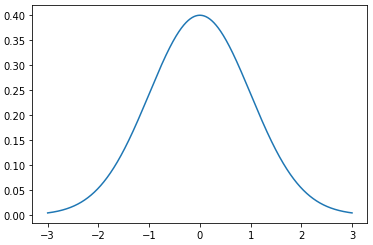
\includegraphics[width=1.0\linewidth]{cap02/distnormal.png}
		\caption{Curva da Distribuição Normal}
		\label{fig:first}
	\end{minipage}\rule{3em}{0pt}%
	\begin{minipage}[t]{0.4\linewidth}
		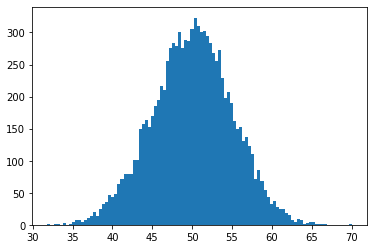
\includegraphics[width=1.0\linewidth]{cap02/distnormalreal.png}
		\caption{A partir de dados randômicos}
		\label{fig:first}
	\end{minipage}\rule{3em}{0pt}%
\end{figure}

Também podemos a partir dessa segunda, calcular seus valores principais:
\begin{lstlisting}
print('Média: %.3f' % np.mean(data))
print('Mediana: %.3f' % np.median(data))
print('Moda:', stats.mode(data))
\end{lstlisting} \vspace{-1em}

\section{Distribuição de Poisson}\index{Conceitos Introdutórios}
Pronuncia-se \textit{Poassom}, é uma distribuição de Probabilidade Discreta para uma variável aleatória X que satisfaça as seguintes condições:
\vspace{-1em}
\begin{itemize}[noitemsep]
	\item O experimento consistem em calcular quantas vezes (k) que um evento ocorre em um dado intervalo.
	\item A probabilidade do evento ocorrer é a mesma em cada intervalo.
	\item O experimento resulta em resultados que podem ser classificados como \textbf{sucessos} ou \textbf{falhas}.
	\item O número médio de sucessos ($\mu$) que ocorre em uma região especificada é conhecido.
	\item A probabilidade de um sucesso ocorrer é proporcional ao tamanho da região.
	\item A probabilidade de um sucesso ocorrer em uma região extremamente pequena é praticamente zero.
	\item O número de ocorrências de um intervalo é independente.
\end{itemize}

Na prática é uma função de ponto percentual, \textit{Poisson} não existe na forma fechada simples é computado numericamente. Essa é uma distribuição discreta, definida apenas para valores inteiros de X, a função de ponto percentual não é suave da mesma forma que a função de ponto percentual normalmente é para uma distribuição contínua. Começamos com a importação das bibliotecas necessárias:
\begin{lstlisting}
import numpy as np
import matplotlib.pyplot as plt
import seaborn as sns
%matplotlib inline
\end{lstlisting}

A NumPy já nos provê a função necessária para vermos como é o gráfico:
\begin{lstlisting}
dp = np.random.poisson(lam=3, size=(1000))
plt.hist(dp)
plt.show()
\end{lstlisting}

Geramos 1.000 números aleatórios com uma ocorrência 3 e obtemos como resultado:
\begin{figure}[H]
	\centering
	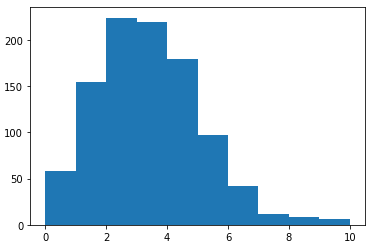
\includegraphics[width=0.5\textwidth]{cap02/distPoisson1.png}
	\caption{Distribuição de Poisson na MatPlotLib}
\end{figure}

Uma variável aleatória de Poisson é o número de sucessos resultantes de um experimento de Poisson. Porém esse gráfico fica bem mais apresentável com o uso da SeaBorn:
\begin{lstlisting}
sns.distplot(dp)
plt.show()
\end{lstlisting}

E obtemos:
\begin{figure}[H]
	\centering
	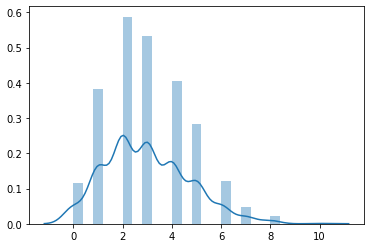
\includegraphics[width=0.5\textwidth]{cap02/distPoisson2.png}
	\caption{Distribuição de Poisson na Seaborn}
\end{figure}

\begin{note}[Historicamente falando] 
	1946, o estatístico britânico \textit{RD Clarke} publicou "\textit{Uma Aplicação da Distribuição de Poisson}", com sua análise dos acertos de bombas voadoras (mísseis V-1 e V-2) em Londres durante a II Guerra Mundial. Algumas áreas foram atingidas com mais frequência do que outras. Os militares britânicos desejavam saber se os alemães estavam atacando esses distritos (os acertos indicavam grande precisão técnica) ou se a distribuição era por acaso. Se os mísseis fossem de fato apenas alvos aleatórios (dentro de uma área mais geral), os britânicos poderiam simplesmente dispersar instalações importantes para diminuir a probabilidade de serem atingidos.
\end{note}

Se acertarmos a escala, surpreendentemente, ao colocar uma Distribuição Normal e uma de Poisson sobrepostas:
\begin{lstlisting}
sns.distplot(np.random.normal(loc=50, scale=7, size=1000), hist=False, label='normal')
sns.distplot(np.random.poisson(lam=50, size=1000), hist=False, label='poisson')
plt.show() 
\end{lstlisting}

Obtemos como resultado:
\begin{figure}[H]
	\centering
	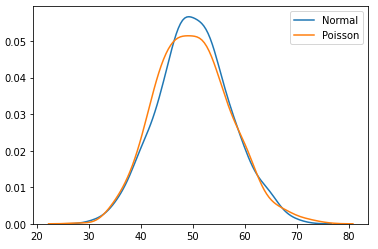
\includegraphics[width=0.4\textwidth]{cap02/distNormalPoisson.png}
	\caption{Distribuição Normal e de Poisson}
\end{figure}

E claramente percebemos a similaridade entre ambas. Um caso curioso que ocorre com a Distribuição de Poisson é a "cauda longa", sabemos que em qualquer comércio existe os produtos que mais possuem saída e aqueles outros que estão ali para "compor estoque". Por exemplo:
\begin{lstlisting}
ax = sns.distplot(np.random.poisson(lam=3, size=10000), bins=27, kde=False)
ax.set(xlabel='Mercadorias', ylabel='Unidades Vendidas')
plt.show()
\end{lstlisting}

Obtemos como resultado:
\begin{figure}[H]
	\centering
	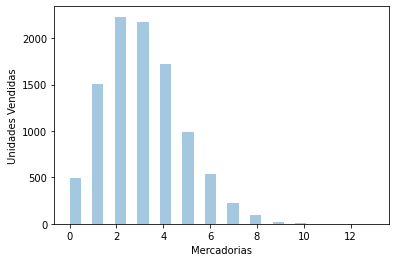
\includegraphics[width=0.4\textwidth]{cap02/distPoissonCauda.png}
	\caption{A Cauda Longa}
\end{figure}

A partir do número 6 temos um decrescimento constante, o que demonstra exatamente o que acontece com algumas mercadorias.

\section{Distribuição Binomial}\index{Conceitos Introdutórios}
Neste tipo de distribuição apenas dois resultados são possíveis: sucesso ou fracasso, ganho ou perda, vitória ou perda e a probabilidade é exatamente a mesma para todas as tentativas. No entanto, os resultados não precisam ser igualmente prováveis, e cada estudo é independente um do outro. Podemos ver sua curva com 1.000 lançamentos de 10 possibilidades
\begin{lstlisting}
sns.distplot(np.random.binomial(n=10, p=0.5, size=1000), hist=True)
plt.show()
\end{lstlisting}

Obtemos como resultado:
\begin{figure}[H]
	\centering
	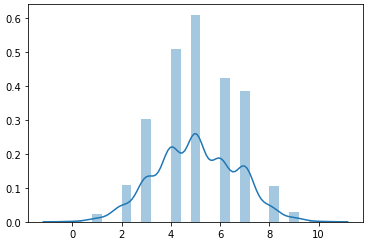
\includegraphics[width=0.45\textwidth]{cap02/distBinomial.png}
	\caption{Distribuição Binomial}
\end{figure}

A principal diferença para a normal é que essa é contínua, enquanto que a binomial é discreta, mas se houver pontos de dados suficientes, serão bastante semelhantes (inclusive com a Poisson).

\begin{lstlisting}
sns.distplot(np.random.normal(loc=50, scale=7, size=1000), hist=False, label='Normal')
sns.distplot(np.random.poisson(lam=50, size=1000), hist=False, label='Poisson')
sns.distplot(np.random.binomial(n=100, p=0.5, size=200), hist=False, label='Binomial')
plt.show()
\end{lstlisting}

Obtemos como resultado:
\begin{figure}[H]
	\centering
	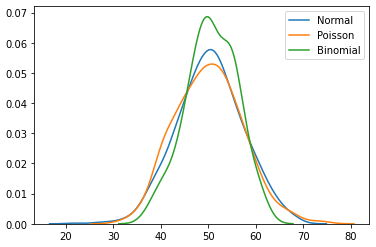
\includegraphics[width=0.45\textwidth]{cap02/distCompara.png}
	\caption{Mesmo gráfico 3 Distribuições}
\end{figure}

Mas e na prática? Imaginemos que 90\% dos passageiros reservados chegam de fato para sua viagem. Suponhamos um transporte que pode conter 45 assentos. Muitas vezes as companhias praticam "excesso de reservas" (conhecido por \textit{Overbooking}) isso significa que vende mais passagens do que os assentos disponíveis. Isso se deve ao fato de que às vezes os passageiros não aparecem um assento vazio representa perda. No entanto, ao reservar em excesso corre o risco de ter mais passageiros do que assentos.

Com esses riscos em mente, uma companhia decide vender mais de 45 bilhetes. Supondo que desejam manter a probabilidade de ter mais de 45 passageiros para embarcar no voo abaixo de 0,4 quantas passagens podem vender?

Para resolvermos isso precisamos da SciPy, e procedemos a seguinte codificação:
\begin{lstlisting}
from scipy.stats import binom_test
for i in range(45, 51):
print(i, "-", binom_test(x=45, n=i, p=0.9, alternative='greater'))
\end{lstlisting}

Obtemos como resultado: \\
\codigo{45 - 0.008727963568087723 \\
	46 - 0.04800379962448249 \\
	47 - 0.13833822255419037 \\
	48 - 0.27986215181073293 \\
	49 - 0.449690866918584 \\
	50 - 0.6161230077242769}

O parâmetro \textit{alternative} que indica a hipótese, podemos usar: \vspace{-1em}
\begin{itemize}[nolistsep]
	\item \textit{greater} maior que
	\item \textit{less} menor que
	\item \textit{two-sided} maior e menor que (valor padrão)
\end{itemize}

E podemos vender \textbf{48 passagens}. E agora sabemos porque todas as companhias de transporte praticam \textit{overbooking}. Para vermos isso graficamente:
\begin{lstlisting}
sns.distplot(np.random.binomial(n=48, p=0.9, size=400), label='Binomial')
\end{lstlisting}

Obtemos como resultado:
\begin{figure}[H]
	\centering
	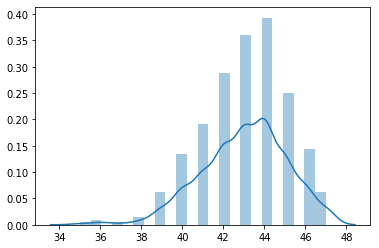
\includegraphics[width=0.45\textwidth]{cap02/overbooking.png}
	\caption{Gráfico do Overbooking}
\end{figure}

\section{Feature Selection}\index{Conceitos Introdutórios}
\textbf{Seleção de Atributos}, Variáveis, Recursos ou Subconjuntos de Variáveis, são os vários nomes para o processo para a seleção de \textit{features} (atributo) relevantes para a construção de modelos. 

\textit{Label} (ou rótulo) é a variável que estamos prevendo, enquanto que uma \textit{feature} é a variável de entrada, que pode inclusive ser mais de uma. Deve ser realizada depois da etapa de pré-processamento dos dados. 

O objetivo é selecionar as melhores variáveis como possíveis \textbf{preditoras}. Essa etapa ajuda a reduzir o \textit{overfitting}, aumenta a acurácia do modelo e reduz o tempo de treinamento.

São os seguintes métodos que podemos utilizar: \vspace{-1em}
\begin{itemize}
	\item \textbf{Filter Methods}: usam medidas estatísticas para atribuir uma pontuação para cada \textit{feature}. Estas são classificadas de modo a serem mantidas ou removidas do modelo. Normalmente usamos testes univariados que consideram a independência da \textit{feature} com a variável alvo. Exemplo: \textit{chi squared}, pontuações com Coeficiente de Correlação.
	\item \textbf{Wrapper Methods}: selecionam um conjunto de \textit{features}, onde diferentes combinações são preparadas, avaliadas e comparadas. Um modelo preditivo é usado para avaliar a combinação de \textit{features} a atribuir uma nota a partir a acurácia de modelo. Exemplo: RFE.
	\item \textbf{Embedded Methods}: aprendem quais \textit{features} contribuem melhor para a acurácia do modelo no momento de sua construção. Exemplo: Métodos de Penalização, Algoritmos Lasso, \textit{Elastic NEt} e \textit{Ridge Regression}.
\end{itemize}

\begin{note}[Bases de Dados] 
	Para TODOS os exemplos neste livro, utilizamos bases de dados que estão disponibilizadas em \url{https://github.com/fernandoans/machinelearning/tree/master/bases}. Salvo qualquer observação em contrário.
\end{note}

Importação das bibliotecas utilizadas:
\begin{lstlisting}
import pandas as pd
from sklearn.feature_selection import SelectKBest
from sklearn.feature_selection import f_classif, mutual_info_classif
from sklearn.feature_selection import chi2
from sklearn.linear_model import LogisticRegression
from sklearn.feature_selection import RFE
from sklearn.ensemble import RandomForestClassifier
%matplotlib inline
\end{lstlisting}

Os classificadores estão contidos na Scikit-Learn e utilizaremos como nossa fonte de dados o arquivo chamado \textbf{pima-indians-diabetes.csv}. Criar um DataFrame para esta:
\begin{lstlisting}
colnames = ['gest', 'glic', 'sang', 'skin', 'insul', 'mass', 'familia', 'idade', 'conf']
df = pd.read_csv('pima-indians-diabetes.csv', names=colnames)
df.head()
\end{lstlisting}

Esta base são dados do \textbf{Instituto Nacional de Diabetes, Doenças Digestivas e Renais} sendo de pacientes do sexo feminino. Consiste de várias variáveis preditivas médicas (independentes) e uma variável alvo (dependente). Variáveis independentes incluem o número de gestações que a paciente teve, seu IMC, nível de insulina, idade e outras informações. Essa base possui 798 linhas sem quaisquer presença de nulos, verificar com:
\codigo{df.info()}

A coluna \textit{conf} é a nossa variável alvo se o paciente em questão teve ou não diabetes, então precisamos isolá-la:
\begin{lstlisting}
X = df.drop(['conf'], axis=1)
y = df['conf']
\end{lstlisting}

Para as outras desejamos sabe: qual (ou quais) variável independente se comportar melhor para o nosso modelo?

\subsection{Coeficientes de Coorelação}\index{Conceitos Introdutórios}
Como primeira forma aplicamos os testes estatísticos:
\begin{lstlisting}
f_classif1 = SelectKBest(score_func=f_classif, k=4)
fit1 = f_classif1.fit(X,y)
\end{lstlisting}

Os tipos para o \textbf{SelectKBest}, neste caso, são: \vspace{-1em}
\begin{itemize}
	\item \textbf{f\_classif}: mais adequado quando os dados são numéricos e a variável alvo é categórica.
	\item \textbf{mutual\_info\_classif}: mais adequando quando não existe uma dependência linear entre os atributos e a variável alvo.
	\item \textbf{f\_regression}: para resolver problemas de regressão.
\end{itemize}

Visualizar as variáveis selecionadas:
\begin{lstlisting}
cols = fit1.get_support(indices=True)
df.iloc[:,cols]
\end{lstlisting}

Indica que número de gestações (\textit{gest}), concentração de glicose no plasma (\textit{glic}), índice de massa corporal (\textit{mass}) e \textit{idade} seriam as melhores candidatas.

\subsection{Chi Squared}\index{Conceitos Introdutórios}
Usada para medir a dependência entre variáveis estocásticas, o uso dessa função "elimina" os recursos com maior probabilidade de serem independentes da classe e, portanto, irrelevantes para a classificação:
\begin{lstlisting}
test2 = SelectKBest(chi2, k=4)
fit2 = test2.fit(X, y)
\end{lstlisting}

Visualizar as variáveis selecionadas:
\begin{lstlisting}
cols = fit2.get_support(indices=True)
df.iloc[:,cols]
\end{lstlisting}

Percebemos que aconteceu uma mudança nas variáveis selecionadas: \textit{glic}, \textit{mass} e \textit{idade} continuam, porém ao invés de \textit{gest} aparece a quantidadde adminstrada de insulina (insul).

\subsection{RFE}\index{Conceitos Introdutórios}
\textit{Recursive Feature Elimination} é um método que remove o(s) recurso(s) mais fraco(s) até que o número especificado de recursos seja atingido. Sendo assim é necessário informar ao RFE o número de atributos caso contrário reduz pela metade esse valor de acordo com o número de \textit{feature} dos dados:
\begin{lstlisting}
model = LogisticRegression(max_iter=2000, solver='lbfgs')
rfe = RFE(model, n_features_to_select=4)
fit3 = rfe.fit(X, y)
\end{lstlisting}

Visualizar as variáveis selecionadas:
\begin{lstlisting}
cols = fit3.get_support(indices=True)
df.iloc[:,cols]
\end{lstlisting}

Como resultado obtemos quase a mesma combinação anterior e aparece mais a variável \textit{familia } que indica se existem casos de diabetes na família.

\subsection{Ensembles Methods}\index{Conceitos Introdutórios}
Métodos de agrupamento\footnote{São métodos que utilizam vários algoritmos de aprendizado para obter um melhor desempenho preditivo.}, como o algoritmo \textit{Random Forest}, podem ser usados para estimar a importância de cada atributo. Retorna um valor para cada atributo, quanto mais alto esse, maior é a importância desse atributo.

Aplicar o algoritmo:
\begin{lstlisting}
model = RandomForestClassifier(n_estimators=10)
model.fit(X, y)
RandomForestClassifier(bootstrap=True, class_weight=None,
  criterion='gini', max_depth=None, max_features='auto',
  max_leaf_nodes=None, min_impurity_decrease=0.0, min_impurity_split=None,
  min_samples_leaf=1, min_samples_split=2,
  min_weight_fraction_leaf=0.0, n_estimators=10,
  n_jobs=None, oob_score=False, random_state=None,
  verbose=0, warm_start=False)
\end{lstlisting}

E podemos gerar uma visualização:
\begin{lstlisting}
feature_importancia = pd.DataFrame(model.feature_importances_,
  index = X.columns, columns=['importancia']).sort_values('importancia', ascending=False)
feature_importancia
\end{lstlisting}

Porém é preferível vê-las através de um gráfico:
\begin{lstlisting}
feature_importancia.plot(kind='bar')
\end{lstlisting}

Obtemos como resultado:
\begin{figure}[H]
	\centering
	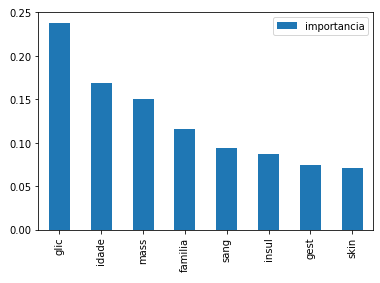
\includegraphics[width=0.5\textwidth]{cap02/acurVariavel.png}
	\caption{Grau de Importância dos Atributos}
\end{figure}

E afinal de contas com tudo o que vimos. Qual Método utilizar?
\begin{itemize}[nolistsep]
	\item Usar \textit{RFE} caso tenha recursos computacionais para isso.
	\item Ao trabalhar com Classificação e as \textit{features} forem numéricas, utilizar \textit{f\_classif} ou \textit{mutual\_info\_classif}.
	\item Ao trabalhar com Regressão e as \textit{features} forem numéricas, utilizar \textit{f\_regression} ou \textit{mutual\_info\_regression}.
	\item Ao trabalhar com \textit{features} categóricos utilizar \textit{Chi Squared}.
\end{itemize}

\section{K Fold Cross Validation}\index{Conceitos Introdutórios}
Vimos como encontrar as melhores \textit{features} para trabalhar, porém verificamos um pequeno problema: qual a forma em se escolher o modelo ideal\footnote{"Ideal" é apenas um conceito para designar qual terá uma melhor acurácia (não usemos como sinônimo para perfeito ou o melhor)} para nossa base de dados? O que fazemos é testar um modelo várias vezes obtendo pedaços diferentes de treino e teste a cada vez.

Usaremos a mesma base de Casos de Diabetes com vários modelos. Começamos com a importação das bibliotecas:
\begin{lstlisting}
from pandas import read_csv
import matplotlib.pyplot as plt
from sklearn.model_selection import KFold
from sklearn.model_selection import cross_val_score
from sklearn.linear_model import LogisticRegression
from sklearn.tree import DecisionTreeClassifier
from sklearn.neighbors import KNeighborsClassifier
from sklearn.discriminant_analysis import LinearDiscriminantAnalysis
from sklearn.naive_bayes import GaussianNB
from sklearn.svm import SVC
%matplotlib inline
\end{lstlisting}

Em seguida colocamos os dados em um DataFrame:
\begin{lstlisting}
colnames = ['gest', 'glic', 'sang', 'skin', 'insul', 'mass', 'familia', 'idade', 'conf']
df = read_csv('pima-indians-diabetes.data.csv', names=colnames)
df.head()
\end{lstlisting}

Para não ficar gerando códigos repetitivos, criar uma lista com todos os modelos que vamos executar:
\begin{lstlisting}
models = []
models.append(('LR', LogisticRegression()))
models.append(('LDA', LinearDiscriminantAnalysis()))
models.append(('KNN', KNeighborsClassifier()))
models.append(('DT', DecisionTreeClassifier()))
models.append(('NB', GaussianNB()))
models.append(('SVM', SVC()))
\end{lstlisting}

Trabalharemos com Regressão Logística (LR), Análise Descriminante (LDA), K-Neighbors (KNN), Árvore de Decisão (DT), Gaussian tipo NB e SVM. E para avaliar a acurácia de cada um dos modelos:
\begin{lstlisting}
acuracia = []
for sigla, modelo in models:
  kfold = KFold(n_splits=10, random_state=7, shuffle=True)
  resultado = cross_val_score(modelo, X, Y, cv=kfold, scoring='accuracy', n_jobs=-1)
  acuracia.append(resultado.mean())
  print("%s: %f (%f)" % (sigla, resultado.mean(), resultado.std())) 
\end{lstlisting}

O objeto \textbf{KFold} criado executa 10 vezes (definido em \textit{n\_splits}) cada um dos modelos mantendo um estado de aleatoriedade de 7 registros. O método \textit{cross\_val\_score} realiza todo o trabalho que tivemos para executar um modelo, dividir a base de dados em treino e teste obtendo o score de cada execução e obtemos o mesmo resultado final, a cada resposta podemos definir o número de vezes a executar (definido em \textit{n\_jobs}) neste caso será executado somente 1 vez (o valor é -1).

Ao mostrar a variável \textit{resultado} obtemos uma lista de 10 valores para cada um dos modelos, porém para facilitar, trazemos a média (que também será adicionada para a lista \textit{acuracia}) e o desvio padrão: \\
\codigo{LR: 0.778640 (0.047350) \\
LDA: 0.766969 (0.047966) \\
KNN: 0.710988 (0.050792) \\
DT: 0.696770 (0.046741) \\
NB: 0.759142 (0.038960) \\
SVM: 0.760458 (0.034712)}

Também podemos ter isso de forma gráfica:
\begin{lstlisting}
fig = plt.figure(figsize = (8,4))
axes = fig.add_axes([0.0, 0.0, 1.0, 1.0])
axes.set_title('Comparação dos Modelos');
axes.bar([item[0] for item in models], acuracia)
plt.show()
\end{lstlisting}

E obtemos como resultado:
\begin{figure}[H]
	\centering
	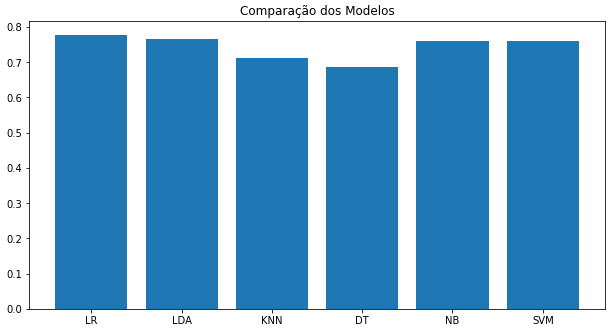
\includegraphics[width=0.5\textwidth]{cap02/acurModelo.png}
	\caption{Melhor Acurácia dos Modelos}
\end{figure}

\section{Matriz de Confusão}
A Matriz de Confusão nos auxilia a medir a precisão do nosso modelo. A acurácia é uma boa medida porém um tanto falha, suponhamos que estejamos para realizar um trabalho com dados de pacientes que desejam saber a possibilidade de desenvolver uma determinada doença ou não. São quatro respostas possíveis que o nosso modelo pode prover: \vspace{-1em}
\begin{itemize}
	\item \textbf{Verdadeiro Positivo} (\textit{TP - true positive}): no conjunto da classe real, o resultado foi correto. O paciente desenvolveu a doença e o modelo previu que iria desenvolver. (T \& T)
	\item \textbf{Falso Positivo} (\textit{FP - false positive}): no conjunto da classe real, o resultado foi incorreto. O paciente desenvolveu a doença e o modelo previu que não iria desenvolver. (T \& F - Erro tipo 2)
	\item \textbf{Falso Negativo} (\textit{FN - false negative}): no conjunto da classe real, o resultado foi incorreto. O paciente não desenvolveu a doença e o modelo previu que iria desenvolver. (F \& T - Erro tipo 1)
	\item \textbf{Verdadeiro Negativo} (\textit{TN - true negative}): no conjunto da classe real, o resultado foi correto. O paciente não desenvolveu a doença e o modelo previu que não iria desenvolver. (F \& F)
\end{itemize}

Os casos 2 e 3 são \underline{erros} no modelo, sendo que o \textbf{2} é é considerado um pior tipo. Para começar com a nossa prática importar as bibliotecas necessárias:
\begin{lstlisting}
import numpy as np
import pandas as pd
import matplotlib.pyplot as plt
import seaborn as sn
from sklearn.model_selection import train_test_split
from sklearn.metrics import confusion_matrix
from sklearn.linear_model import LogisticRegression
%matplotlib inline
\end{lstlisting}

A biblioteca \textit{sklearn.metrics} na versão 0.22 ganhou o método \textbf{confusion\_matrix}. Somente para entendermos como funciona a Matriz de Confusão, suponhamos que foi realizado um teste com base em características de pacientes, existe uma possibilidade de desenvolver (D) ou não (S) uma determinada doença:
\begin{lstlisting}
y_true = pd.Series(['D','D','D','D','D','D','S','S','S','S','S','S','S'])
y_pred = pd.Series(['D','D','S','D','D','D','D','S','D','S','S','D','S'])
\end{lstlisting}

A série contendo y\_true é o resultado real (ou verdadeiro) e y\_pred foi o resultado que o modelo disse que iria ocorrer. Se fossemos somente pela acurácia obtemos 13 respostas sendo 4 delas erradas, porém como saber se o modelo está realmente agindo bem e o mais importante onde está se confundindo?
\begin{lstlisting}
conf = confusion_matrix(y_true, y_pred)
print(conf)
\end{lstlisting}

Ao usarmos o método \textit{confusion\_matrix} obtemos a seguinte Matriz que nos auxilia a responder essas questões: \\
\codigo{$[[$5 1$][$3 4$]]$}

O eixo \textbf{X} da Matriz representa o que foi predito e \textbf{y} o que realmente aconteceu pelo modelo. Nas diagonais obtemos as corretas, cinco que estão Doentes e quatro que estão sadios e o modelo acertou. Porém, três não estão doentes mas foi previsto que estariam (se pensarmos a notícia não é tão ruim - do ponto de vista para o paciente, por isso esse é o erro tipo 1) e um está doente porém prevemos que não estaria (péssima notícia, por isso esse é o erro tipo 2). Visualizar resultados assim pode ser bem complexo, então tentemos uma adaptação do Mapa de Calor da biblioteca \textbf{SeaBorn}:
\begin{lstlisting}
data = {
  'Ocorreu': y_true,
  'Predito': y_pred
}
df = pd.DataFrame(data, columns=['Ocorreu','Predito'])
conf = pd.crosstab(df['Ocorreu'], df['Predito'], rownames=['Ocorreu'], colnames=['Predito'])
res = sn.heatmap(conf, annot=True, fmt='.0f', annot_kws={"size":12}, cmap=plt.cm.Blues)
plt.show()
\end{lstlisting}

E obtemos como resultado:
\begin{figure}[H]
	\centering
	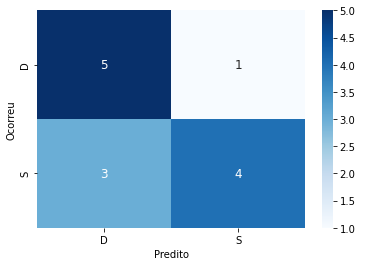
\includegraphics[width=0.45\textwidth]{cap02/matrizConf1.png}
	\caption{Mapa de Calor mostrando a Matriz de Confusão}
\end{figure}

Quanto mais escuro, maior a quantidade de elementos, assim podemos rapidamente avaliar como nosso modelo se comporta (o ideal é que as diagonais fiquem bem escuras enquanto que as extremidades claras).

\subsection{Em valor ou percentual?}
Um detalhe muito comum de acontecer é: devemos mostrar o valor em decimal ou percentual? Ou seja as quantidades reais das amostras ou um percentual do todo? Usar o seguinte código para gerar uma matriz de um teste realizado com imagens:
\begin{lstlisting}
conf_arr = np.array([[88,14,4],[12,85,11],[5,15,91]])
sum = conf_arr.sum()
df_cm = pd.DataFrame(conf_arr,
  index = [ 'Cão', 'Gato', 'Coelho'],
  columns = ['Cão', 'Gato', 'Coelho'])
res = sn.heatmap(df_cm, annot=True, vmin=0.0, vmax=100.0, cmap=plt.cm.Blues)
plt.yticks([0.5,1.5,2.5], ['Cão', 'Gato', 'Coelho'],va='center')
plt.title('Matriz de Confusão')
plt.show()
\end{lstlisting}

E obtemos como resultado:
\begin{figure}[H]
	\centering
	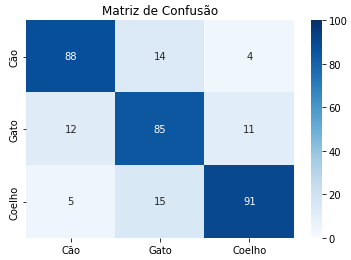
\includegraphics[width=0.5\textwidth]{cap02/matrizConf2.png}
	\caption{Comparativo numérico na Matriz de Confusão}
\end{figure}

E ao realizarmos um ajuste:
\begin{lstlisting}
conf_arr = conf_arr * 100.0 / ( 1.0 * sum )
conf_arr /= 100
df_cm = pd.DataFrame(conf_arr,
  index = [ 'Cão', 'Gato', 'Coelho'],
  columns = ['Cão', 'Gato', 'Coelho'])
res = sn.heatmap(df_cm, annot=True, vmin=0.0, vmax=0.3, fmt='.2%', cmap=plt.cm.Blues)
plt.title('Matriz de Confusão (em %)')
plt.show()
\end{lstlisting}

Obtemos a seguinte matriz agora com o resultado em percentual:
\begin{figure}[H]
	\centering
	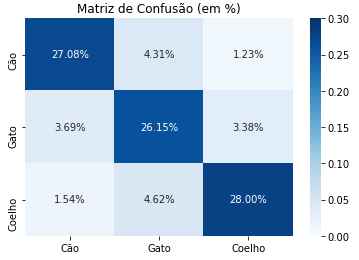
\includegraphics[width=0.55\textwidth]{cap02/matrizConf3.png}
	\caption{Comparativo percentual na Matriz de Confusão}
\end{figure}

Qual dos dois é melhor? A resposta seria: que fica mais fácil para que o Cientista de Dados consiga explicar o resultado para seu público com a maior clareza, não existe uma regra definida para isso. 

\subsection{Na prática}
Voltamos ao nossos dados sobre Diabetes, ler os dados:
\begin{lstlisting}
colnames = ['gest', 'glic', 'sang', 'skin', 'insul', 'mass', 'familia', 'idade', 'conf']
df = pd.read_csv('pima-indians-diabetes.data.csv', names=colnames)
df.head()
\end{lstlisting}

Deixar somente as colunas que nos interessam, conforme vimos na seleção de atributos:
\begin{lstlisting}
df = df.drop(columns=['sang'],axis=1)
df = df.drop(columns=['insul'],axis=1)
df = df.drop(columns=['gest'],axis=1)
df = df.drop(columns=['skin'],axis=1)
df.head()
\end{lstlisting}

\begin{note}[100\% de Precisão] 
	Sempre que ocorrer 100\% podemos ligar todas as antenas pois existe um erro, nenhum modelo possui essa previsão tão perfeita. Considere também que abaixo de 70\% não é preditivo.
\end{note}

Agora acontece um erro clássico, a base contém \textit{conf} que é nossa variável alvo. Sse seguimos em frente para separar as bases em teste e treino o modelo provavelmente acusa uma acurácia (errada) de 100\% de precisão, é como se ele estivesse colando as respostas. Então devemos isolar essa coluna e retirá-la dos dados. 
\begin{lstlisting}
conf = df['conf']
df = df.drop(columns=['conf'],axis=1)
\end{lstlisting}

E assim podemos separar a base de dados em treino e teste:
\begin{lstlisting}
X_train, X_test, y_train, y_test = train_test_split(df, conf, test_size = .25)
\end{lstlisting}

Usamos uma medida de 25\%, ou seja 75\% para treino e o restante para testar nosso modelo. Existem 768 registros não nulos no total, o resultado será: 576 registros para o modelo treinar e 192 para testar. Normalmente deixamos 25\% para teste e verificação da acurácia do modelo esse número pode ser aumentado ou diminuído conforme seus dados, não existe uma regra definida.

Conforme nossa verificação do melhor modelo, vimos que devemos trabalhar com \textbf{Regressão Logística}, então executar o modelo e verificar a acurácia:
\begin{lstlisting}
clf = LogisticRegression(max_iter=10000)
clf.fit(X_train, y_train)
print('Acurácia:', clf.score(X_test, y_test))
\end{lstlisting}

Esse resultado pode variar mas está em torno dos 76\%, o problema é, onde esse modelo está errando? Executar a matriz de confusão para descobrir:
\begin{lstlisting}
y_pred = clf.predict(X_test)
conf = confusion_matrix(y_test, y_pred)
data = {
  'Ocorreu': y_test,
  'Predito': y_pred
}
df2 = pd.DataFrame(data, columns=['Ocorreu','Predito'])
conf = pd.crosstab(df2['Ocorreu'], df2['Predito'], rownames=['Ocorreu'], colnames=['Predito'])
res = sn.heatmap(conf, annot=True, fmt='.0f', annot_kws={"size":12}, cmap=plt.cm.Blues)
plt.show()
\end{lstlisting}

E obtemos como resultado:
\begin{figure}[H]
	\centering
	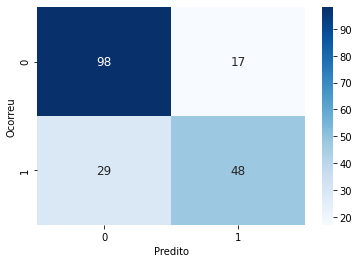
\includegraphics[width=0.4\textwidth]{cap02/matrizConf4.png}
	\caption{Resultado da Matriz de Confusão}
\end{figure}

Vemos que o modelo se comporta bem nos casos que o paciente não tem diabetes, acerta 85,2\% e erra 14,8\% das vezes. Já quando tem a doença acerta 62,3\% e erra 37,7\% das vezes. Ou seja, para melhorarmos a acurácia precisamos de mais dados com pacientes que desenvolveram a diabetes.

\section{Curva ROC e Valor AUC}
Entre todas as teorias vistas para Ciência de Dados este é um dos conceitos mais simples e ao mesmo tempo mais complicado (acho que é equivalente a Matriz de Confusão e inclusive depende dela).

Na teoria \textbf{ROC} (\textit{Receiver Operating Characteristic}, algo como Característica de Operação do Receptor) é uma curva de probabilidade. É criada ao traçar a taxa de verdadeiro-positivo (TPR - true positive rate) contra a taxa de falsos-positivos (FPR - false positive rate). Que taxas são essas? Voltando ao conceito de Matriz de Confusão a TPR e FPR são calculadas pelas fórmulas:
\begin{figure}[H]
	\centering
	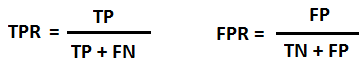
\includegraphics[width=0.4\textwidth]{cap02/ROCeAUCformulas.png}
	\caption{Fórmulas para o cálculo da ROC}
\end{figure}

Ou seja, número de vezes que o classificador acertou a predição contra o número de vezes que errou. \textbf{AUC} (\textit{Area Under the Curve}) representa a área da ROC, considera-se como o grau ou medida de separabilidade. Quanto maior o valor, melhor é o modelo em prever ou (por exemplo) em distinguir entre pacientes com e sem uma determinada doença.
\begin{figure}[H]
	\centering
	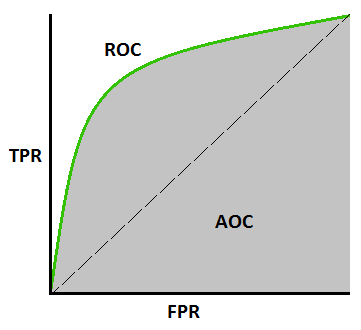
\includegraphics[width=0.35\textwidth]{cap02/ROCeAUCvisao.png}
	\caption{Fórmulas para o cálculo da ROC}
\end{figure}

Vejamos um simples exemplo para entendermos como esse processo funciona:
\begin{lstlisting}
import pandas as pd
from sklearn import metrics
from sklearn.model_selection import train_test_split
import matplotlib.pyplot as plt
from sklearn.model_selection import cross_val_score
from sklearn.datasets import make_classification
from sklearn.linear_model import LogisticRegression
from sklearn.ensemble import RandomForestClassifier
%matplotlib inline
\end{lstlisting}

Apenas para entendermos como aquilo tudo que foi escrito no início da seção funciona, usar a função \textit{make\_classification} para produzir alguns dados aleatórios:
\begin{lstlisting}
X, y = make_classification(n_samples = 10000, n_features=10, n_classes = 2, flip_y = 0.5)
X_train, X_test, y_train, y_test = train_test_split(X, y, test_size = .25)
\end{lstlisting}

Foram geradas 10.000 amostras com 10 campos e 2 classes (traduzindo para o português isso significa valores 0 e 1), separamos 25\% para testar nosso modelo. Usar o Modelo de Regressão Logística para analisar esses dados:
\begin{lstlisting}
model = LogisticRegression(solver='liblinear', penalty='l2', C=0.1)
model.fit(X_train, y_train)
print('Acurácia', model.score(X_test, y_test))
\end{lstlisting}

Como os dados são randômicos o resultado pode variar, mas chegamos em torno de 70\%. E agora podemos calcular o \textbf{AUROC} (\textit{Area Under the Receiver Operation Characteristics}):
\begin{lstlisting}
y_prob = model.predict_proba(X_test)[::,1]
fpr, tpr, _ = metrics.roc_curve(y_test, y_prob)
auroc = float(format(metrics.roc_auc_score(y_test, y_prob), '.8f'))
print(auroc)
\end{lstlisting}

Existe 72\% de área preenchida. Qual o motivo da diferença? Estamos levando em consideração as taxas TPR e FPR, não apenas acertou/errou. \textbf{AUC} resume a curva \textbf{ROC} num único valor que é o calculo da “área sob a curva”, porém apresentar a informação assim não tem graça, colocar de forma gráfica:
\begin{lstlisting}
plt.plot(fpr, tpr, label='Curva ROC (area = %0.2f)' % auroc)
plt.plot([0, 1], [0, 1], 'k--')
plt.xlabel('Taxa de Falso Positivo')
plt.ylabel('Taxa de Verdadeiro Positivo')
plt.title('Exemplo do ROC')
plt.legend(loc="lower right")
plt.show()
\end{lstlisting}

E obtemos como resultado:
\begin{figure}[H]
	\centering
	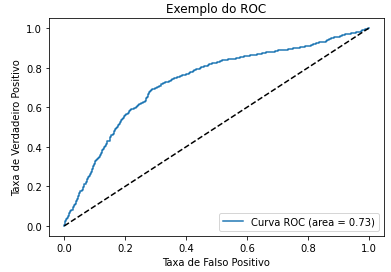
\includegraphics[width=0.45\textwidth]{cap02/ROCeAUCexemplo.png}
	\caption{Visão da ROC}
\end{figure}

\subsection{Na prática}
Voltamos ao nossos dados sobre Diabetes, ler os dados:
\begin{lstlisting}
colnames = ['gest', 'glic', 'sang', 'skin', 'insul', 'mass', 'familia', 'idade', 'conf']
df = pd.read_csv('pima-indians-diabetes.data.csv', names=colnames)
df.head()
\end{lstlisting}

Deixar somente as colunas que nos interessam, conforme vimos na seleção de atributos:
\begin{lstlisting}
df = df.drop(columns=['sang'],axis=1)
df = df.drop(columns=['insul'],axis=1)
df = df.drop(columns=['gest'],axis=1)
df = df.drop(columns=['skin'],axis=1)
df.head()
\end{lstlisting}

Isolar a coluna alvo e retirá-la dos dados. 
\begin{lstlisting}
conf = df['conf']
df = df.drop(columns=['conf'],axis=1)
\end{lstlisting}

Separar a base de dados em treino e teste:
\begin{lstlisting}
X_train, X_test, y_train, y_test = train_test_split(df, conf, test_size = .25)
\end{lstlisting}

Iremos testar dois modelos de agrupamento para saber qual o melhor comportamento com esses dados. Para facilitar nossa vida, criar um método que retorna a acurácia de um determinado modelo:
\begin{lstlisting}
def score(mdl, Xtrn, Xtst, ytrn, ytst):
  mdl.fit(Xtrn, ytrn)
  return float(format(mdl.score(Xtst, ytst), '.8f'))
\end{lstlisting}

Recebemos o modelo a ser treinado, e o conjunto de variáveis X e y de treino e teste para devolvermos a acurácia do modelo. De modo semelhante:
\begin{lstlisting}
def auroc(ytst, yprob):
  fpr, tpr, _ = metrics.roc_curve(ytst, yprob)
  auc = float(format(metrics.roc_auc_score(ytst, yprob), '.8f'))
  return fpr, tpr, auc 
\end{lstlisting}

Esse outro método recebe o y de teste e o de probabilidades e retorna o \textbf{FPR}, \textbf{TPR} e \textbf{AUC}.

Os modelos de agrupamento para realizarmos nosso teste são \textbf{Regressão Logística} e \textbf{Floresta Aleatória}. Para cada um desses, basicamente, são os mesmos comandos.

\textbf{Regressão Logística}:
\begin{lstlisting}
clfRL = LogisticRegression(max_iter=1000)
print("Acurácia RL:", score(clfRL, X_train, X_test, y_train, y_test))
y_probRL = clfRL.predict_proba(X_test)[::,1]
fprRL, tprRL, aucRL = auroc(y_test,  y_probRL)
print("AUC RL", aucRL)
\end{lstlisting}

\textbf{Floresta Aleatória}:
\begin{lstlisting}
clfRF = RandomForestClassifier(n_estimators=1000)
print("Acurácia RF:", score(clfRF, X_train, X_test, y_train, y_test))
y_probRF = clfRF.predict_proba(X_test)[::,1]
fprRF, tprRF, aucRF = auroc(y_test,  y_probRF)
print("AUC RF:", aucRF)
\end{lstlisting}

Ambos os modelos trabalham com grupos de 1.000, sendo que para a \textbf{Regressão Logística} isso é considerado de iterações realizadas enquanto que para a \textbf{Floresta Aleatória} o número de árvores de decisão utilizadas. 

\begin{note}[Como esses modelos trabalham?] 
	Não devemos nos preocupar nesse momento como esses modelos processam, em capítulos subsequentes trataremos separadamente cada um deles. Aqui veremos apenas os conceitos que serão necessários para a melhor escolha e avaliação dos modelos.
\end{note}

E obtemos o seguinte resultado, que pode variar de acordo com o que foi separado de treino e teste: A \textbf{Regressão Logística} atingiu um resultado melhor tanto na acurácia (73,95\%) quanto na curva com quase 80\% de área ocupada enquanto que a \textbf{Floresta Aleatória} ficou com quase 71\% de acurácia e 77,35\% de área. Às vezes o resultado de acurácia pode até ser similar, mas raramente a área ocupada será igual:
\begin{lstlisting}
plt.plot([0, 1], [0, 1], 'k--')
plt.plot(fprRL,tprRL,label="RL " + str(aucRL))
plt.plot(fprRF,tprRF,label="RF " + str(aucRF))
plt.xlabel('Taxa de Falso Positivo')
plt.ylabel('Taxa de Verdadeiro Positivo')
plt.title('Detecção da Diabetes')
plt.legend(loc="lower right")
plt.show()
\end{lstlisting}

E obtemos como resultado:
\begin{figure}[H]
	\centering
	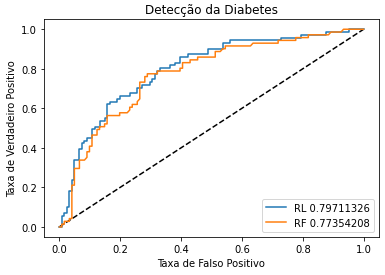
\includegraphics[width=0.45\textwidth]{cap02/ROCeAUCpratica.png}
	\caption{Performance dos Modelos}
\end{figure}

\section{Terminamos?}
Como conceitos sim, mas como prática permita-me deixar um exercício. A \textbf{Scikit-Learn} nos oferece uma base sobre de cistos (Câncer de Mama) encontrados em pacientes de \textit{Wisconsin} com classificação se é malígno (212 amostras) ou benigno (357 amostras). Para usá-la importar a biblioteca:
\begin{lstlisting}
from sklearn.datasets import load_breast_cancer
\end{lstlisting}

Carregamos os dados:
\begin{lstlisting}
cancer = load_breast_cancer()
\end{lstlisting}

E obtemos um objeto \textit{Bunch} da Scikit-Learn com os 569 casos registrados. Para criar as nossas bases de treino e teste usar o comando:
\begin{lstlisting}
X_train, X_test, y_train, y_test = train_test_split(cancer.data, cancer.target, test_size = .25)
\end{lstlisting}

A variável \textit{data} contém os \textit{features} enquanto que \textit{target} se a paciente teve um tipo malígno ou não. Pronto, agora é com você. Aplicar os conhecimentos que vimos nesse capítulo para definir quais são as melhores \textit{features} a usar e o modelo colhendo todos os resultados possíveis.

No endereço \url{https://scikit-learn.org/stable/modules/generated/sklearn.datasets.load_breast_cancer.html} está disponibilizada a documentação sobre esta base.